\documentclass[UTF8]{ctexart}

\usepackage{ulem}
\usepackage{geometry}
\usepackage{amsmath}
\usepackage{multicol}
\usepackage{array}
\usepackage{graphicx}
\usepackage{tabularray}

\title{新东方地理笔记}
\author{Cicada000}
\date{转录开始于2022.6.25}
\geometry{a4paper,right=2.0cm,left=2.0cm,top = 2.0cm, bottom = 2.0cm}

\begin{document}
    
    \maketitle

    这篇地理笔记来自同学的新东方复习资料,内容较为完善但是比较杂乱,还有一些记忆技巧,适合在考前有大量复习时间的时候进行阅读。感谢我的同学提供了新东方的相关资料。

    \thispagestyle{empty}

    \newpage

    \setcounter{page}{1}

    \section*{常见天气系统——锋面系统}

    \[
        \textbf{常见天气系统}
        \begin{cases}
            \text{锋面系统}\\
            \text{低气压、高气压系统}\\
            \text{锋面气旋系统}
        \end{cases}
    \]
    
    \subsection*{锋面系统与天气}

    \begin{table}[h]
        \begin{center}
            \begin{tabular}{ |c|c|c|c|c| }
                \hline 气团分类 & 温度 & 湿度 & 气压 & 密度 \\
                \hline 冷气团 & 低 & 小 & 高 & 大 \\
                \hline 暖气团 & 高 & 大 & 低 & 小 \\
                \hline
            \end{tabular}
        \end{center}
    \end{table}

    \text{对流层中冷暖气团相互运动形成的交界面,称为锋面,主要分为冷锋、暖锋和准静止锋。}

    \subsection*{特点}
    \text{一般冷气团在锋面之下,暖气团在锋面之上。锋面是产生云、雨、大风的原因之一。}\\
    \textbf{冷锋:}
    \text{暖风被迫上升,降水形成在锋后。带来强降水,暴雨等天气。}\\
    \textbf{暖锋:}
    \text{暖气团主动向上爬升,形成锋前降水,多以连续性降水为主。}\\
    \textbf{无论冷锋、暖锋还是准静止锋,降水永远在冷气团一侧。}

    \begin{figure}[h]
        \centering
        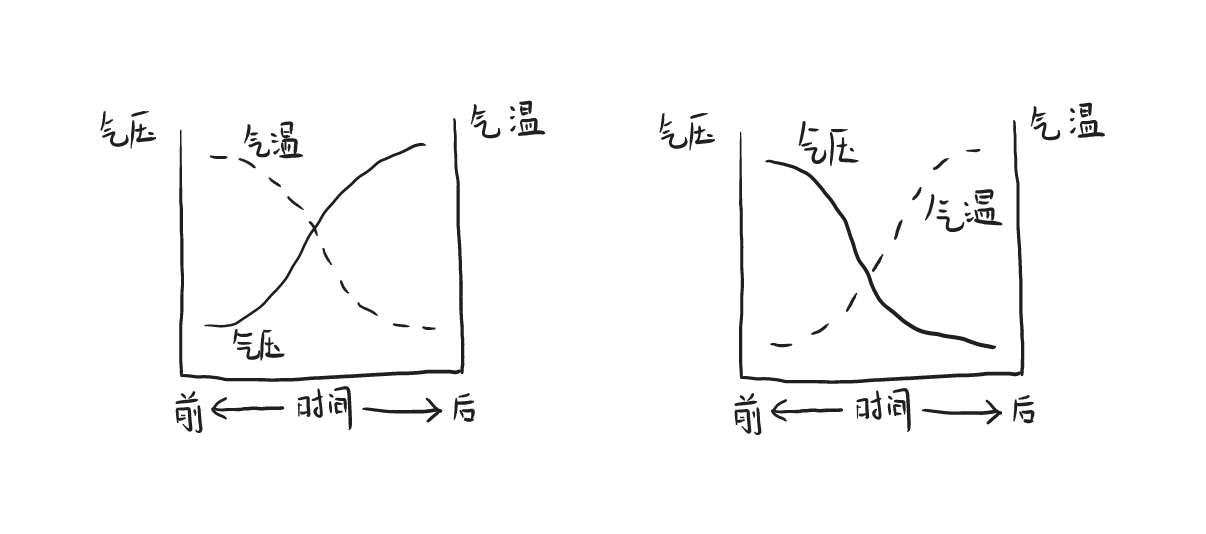
\includegraphics[width=15cm]{img/1-1.png}
        \caption{冷暖锋过境气温气压曲线图}
    \end{figure}

    \subsection*{冷锋}
    \noindent
    \textbf{过境前:}
    \text{单一暖气团控制,温暖晴朗}\\
    \textbf{过境时:}
    \text{冷气团插入暖气团下面,暖气团被抬升,逐渐冷却,出现阴天、刮风、雨、雪、降温等天气。}\\
    \textbf{过境后:}
    \text{冷气团代替原来暖气团位置,气温和湿度下降,气压升高,天气转晴。}\\

    \noindent
    \textbf{降水时间:}
    \text{时间短,强度大}\\
    \textbf{降水位置:}
    \text{在锋后及锋面附近,主要在锋后。}\\
    \textbf{天气实例:}
    \text{我国北方夏季的暴雨,秋冬季爆发的寒潮,北方冬春的大风和沙尘暴,“一场秋雨一场寒”。}

    \subsection*{暖锋}
    \noindent
    \textbf{过境前:}
    \text{单一冷气团控制,低温晴朗}\\
    \textbf{过境时:}
    \text{暖气团沿冷气团徐徐爬升冷却凝结产生连续性降水天气。}\\
    \textbf{过境后:}
    \text{暖气团代替原来冷气团位置,气温和湿度上升,气压降低,天气转晴。}\\

    \noindent
    \textbf{降水时间:}
    \text{时间长,强度小}\\
    \textbf{降水位置:}
    \text{锋前}\\
    \textbf{天气实例:}
    \text{华南地区:春暖多晴,春寒雨起。“一场春雨一场暖”。}

    \subsection*{准静止锋}
    \noindent
    \text{冷暖气团实力相当,移动缓慢而呈准静止状态。}\\
    \textbf{过境时:}
    \text{降水强度小,多连续性降水天气。}\\
    \textbf{我国四大准静止锋:}
    \text{江淮准静止锋、华南准静止锋、云贵准静止锋、天山准静止锋}

    \subsection*{云贵准静止锋}

    \begin{table}[h]
        \begin{center}
            \begin{tabular}{ |c|c| }
                \hline 时间 & 冬春季 \\
                \hline 成因 & 西南季风与南下势力削弱的东北季风影响 \\
                \hline 范围 & 云贵高原 \\
                \hline 影响 & 导致西南地区出现寒潮天气,贵阳地区出现降水 \\
                \hline
            \end{tabular}
        \end{center}
    \end{table}

    \subsection*{天山准静止锋}

    \begin{table}[h]
        \begin{center}
            \begin{tabular}{ |c|c| }
                \hline 时间 & 冬季 \\
                \hline 成因 & 冷锋受到天山阻挡、移动速度减慢 \\
                \hline 范围 & 天山 \\
                \hline 影响 & 造成阴雾、微雪天气,使天山北部与北疆降水增加 \\
                \hline
            \end{tabular}
        \end{center}
    \end{table}

    \subsection*{江淮准静止锋}

    \begin{table}[h]
        \begin{center}
            \begin{tabular}{ |c|c| }
                \hline 时间 & 6、7月 \\
                \hline 成因 & 太平洋暖空气团与江淮流域的冷空气相遇 \\
                \hline 范围 & 长江中下游和淮河流域 \\
                \hline 影响 & 形成连绵阴雨的“梅雨”天气 \\
                \hline
            \end{tabular}
        \end{center}
    \end{table}
    
    \newpage

    \subsection*{华南准静止锋}

    \begin{table}[h]
        \begin{center}
            \begin{tabular}{ |c|c| }
                \hline 时间 & 多出现于冬春两季和秋末 \\
                \hline 成因 & 冷空气南下后势力减弱和南岭山脉的阻挡 \\
                \hline 范围 & 主要活动于南岭山脉和南海地区 \\
                \hline 影响 & 长时间降水 \\
                \hline
            \end{tabular}
        \end{center}
    \end{table}

    \subsection*{如何判断冷锋与暖锋}
    \noindent
    \textbf{1、看符号}\\
    \textbf{2、看冷气团运动方向}\\
    \textbf{3、看锋面坡度}\\
    \textbf{4、看降水区的位置}\\
    \textbf{5、看过境前后气压、气温变化}

    \subsection*{我国锋面雨带移动规律}

    \begin{figure}[h]
        \centering
        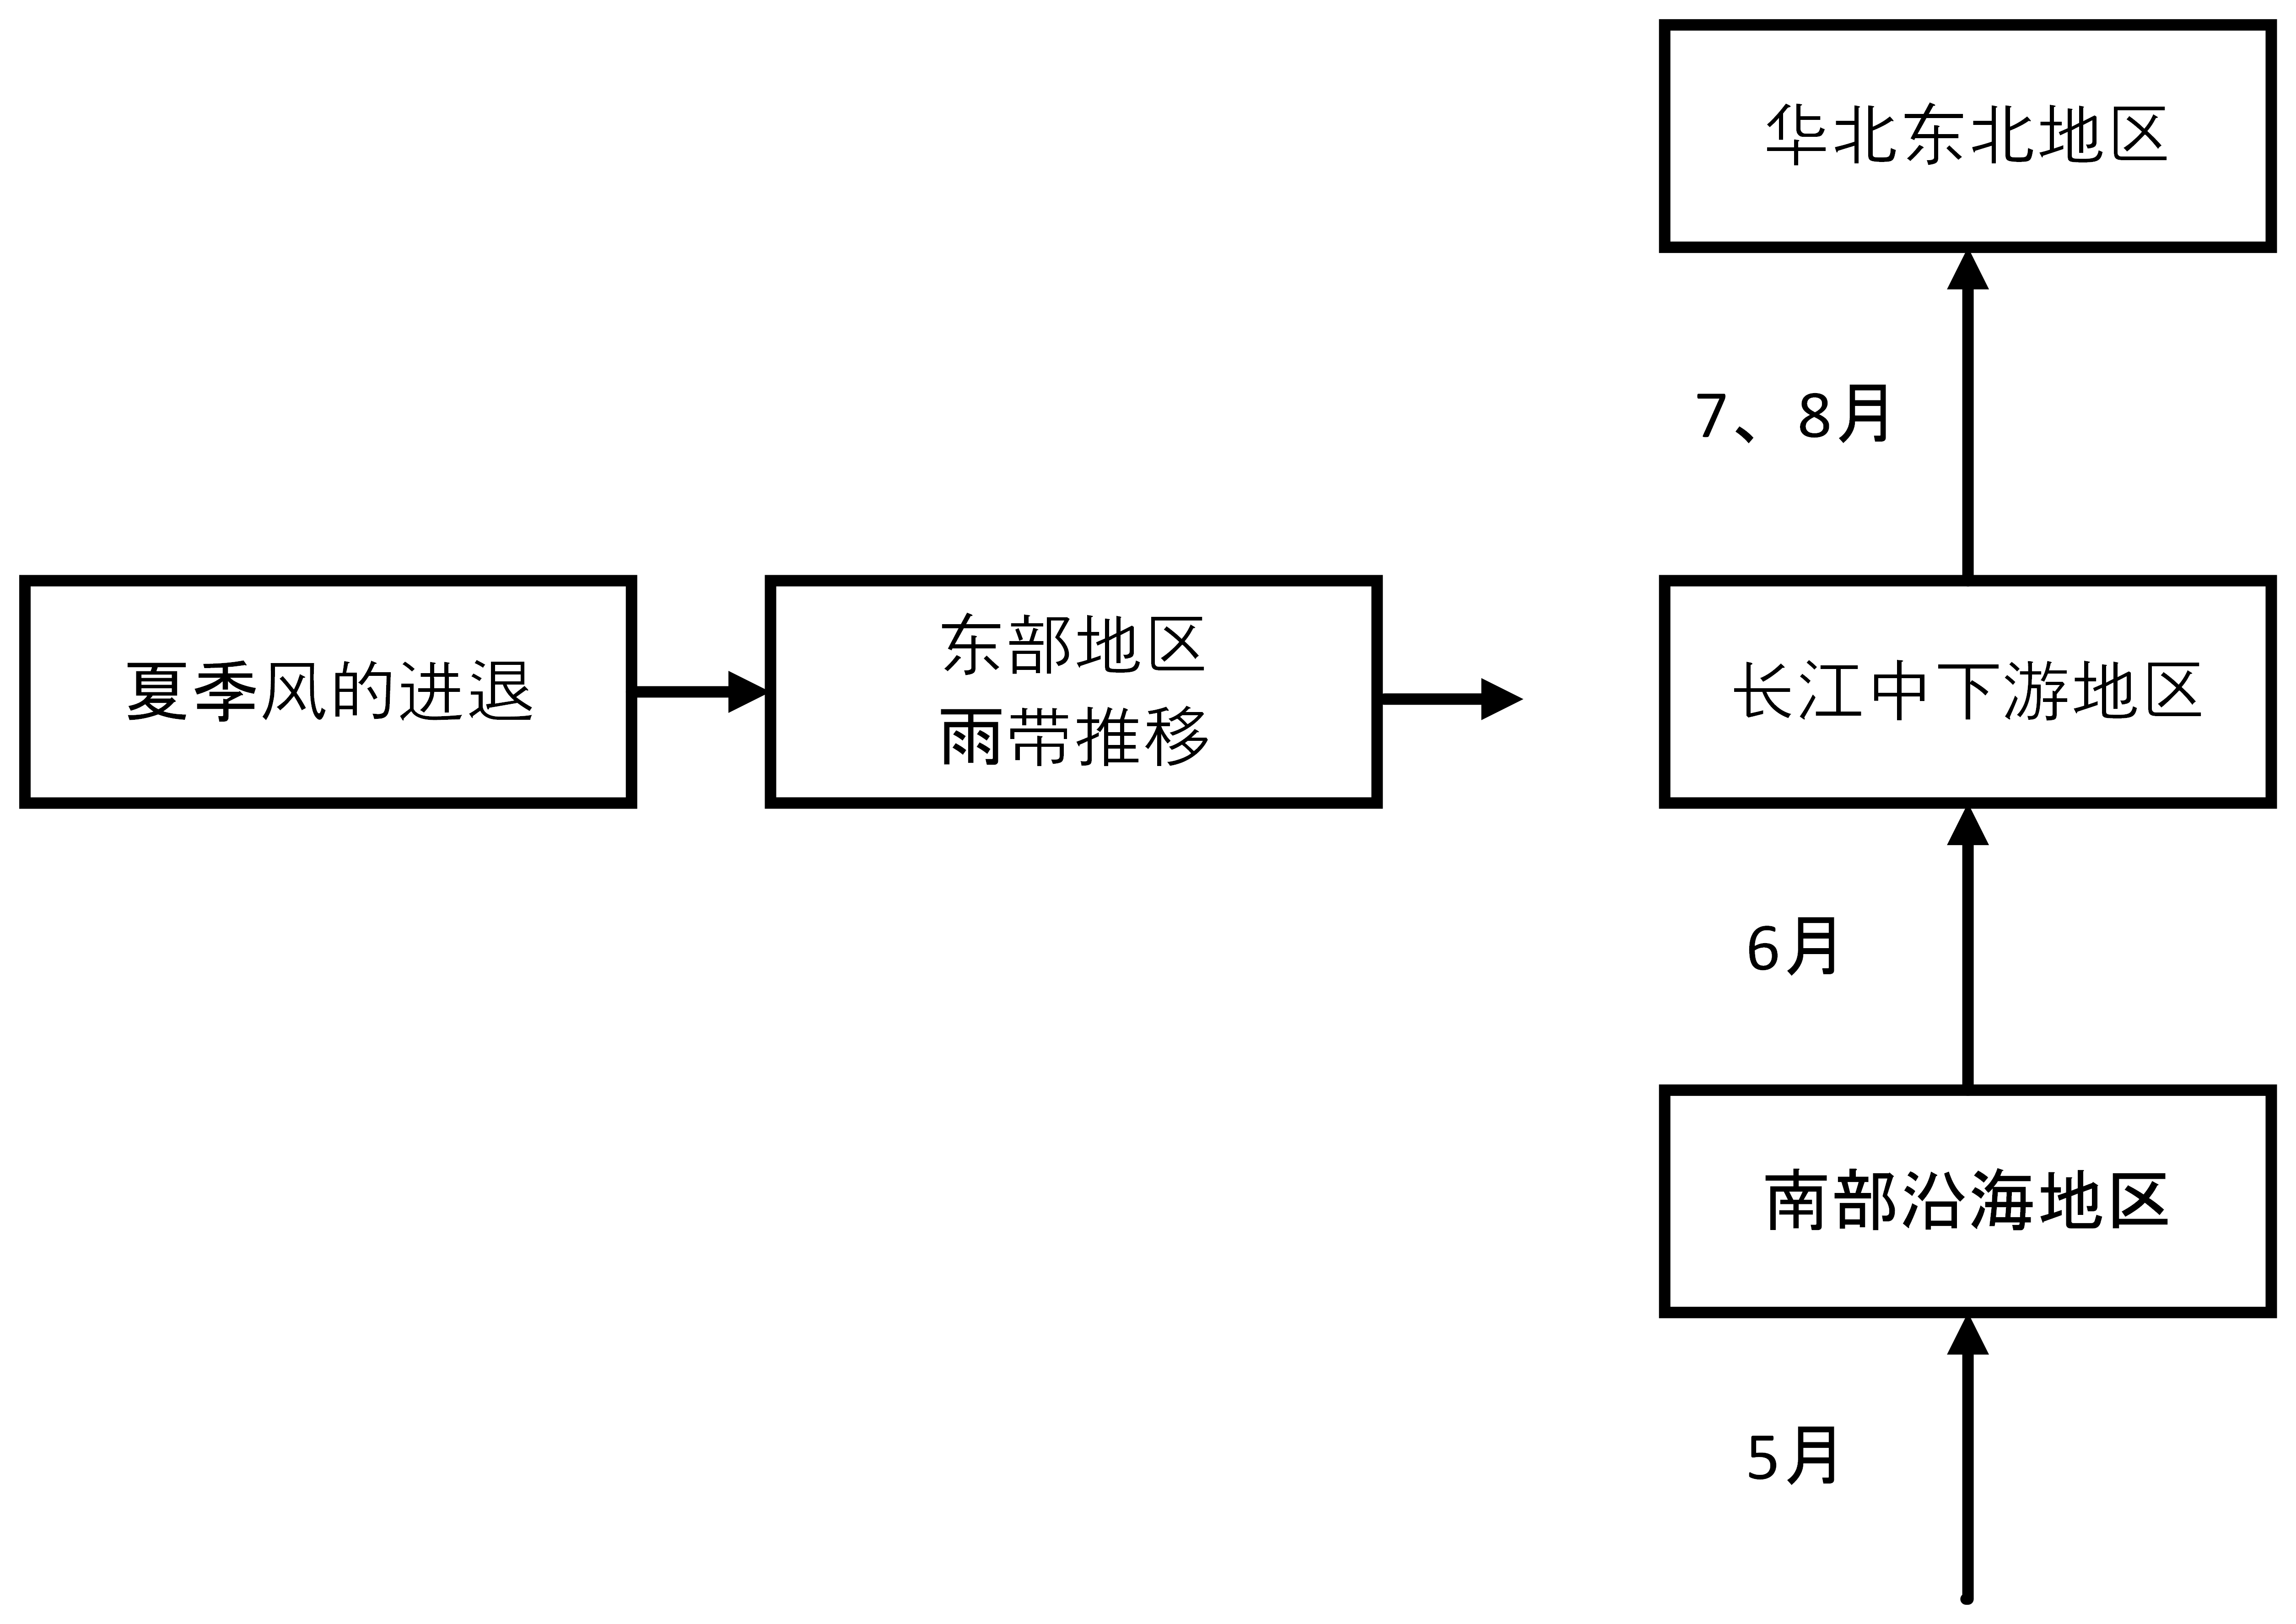
\includegraphics[width=10cm]{img/1-2.png}
        \caption{我国东部地区主要雨带示意图}
    \end{figure}

    \begin{table}[h]
        \begin{center}
            \begin{tabular}{ |c|c|c|c| }
                \hline 时间 & 雨带位置 & 天气系统 & 天气现象 \\
                \hline 3-5月 & 华南地区 & 暖锋 & 华南暴雨 \\
                \hline 6月 & 江淮地区 & 准静止锋 & 梅雨 \\
                \hline 7、8月 & 华北、东北地区 & 冷锋 & 华北暴雨,长江中下游“伏旱” \\
                \hline 9月 & 雨带退回江淮 & 冷锋 & 江淮秋雨连绵 \\
                \hline 10月 & 雨带退回华南 & 冷锋 &  \\
                \hline
            \end{tabular}
        \end{center}
    \end{table}

    \noindent
    \textbf{北方雨季:}
    \text{开始迟,结束早,雨季短。}\\
    \textbf{南方雨季:}
    \text{开始早,结束迟,雨季长。}\\
    \textbf{总结:}
    \text{推进原因是由于副热带高压带的北移,南撤原因是由于副高势力的减弱和北方冷空气的南下。}\\
    \textbf{规律:}
    \text{夏季风势力强,锋面移动快,我国易出现南旱北涝,夏季风势力弱则反之。}

    \newpage

    \section*{常见天气系统——高、低压系统}

    \subsection*{低气压、高气压与气旋、反气旋}

    \begin{figure}[h]
        \centering
        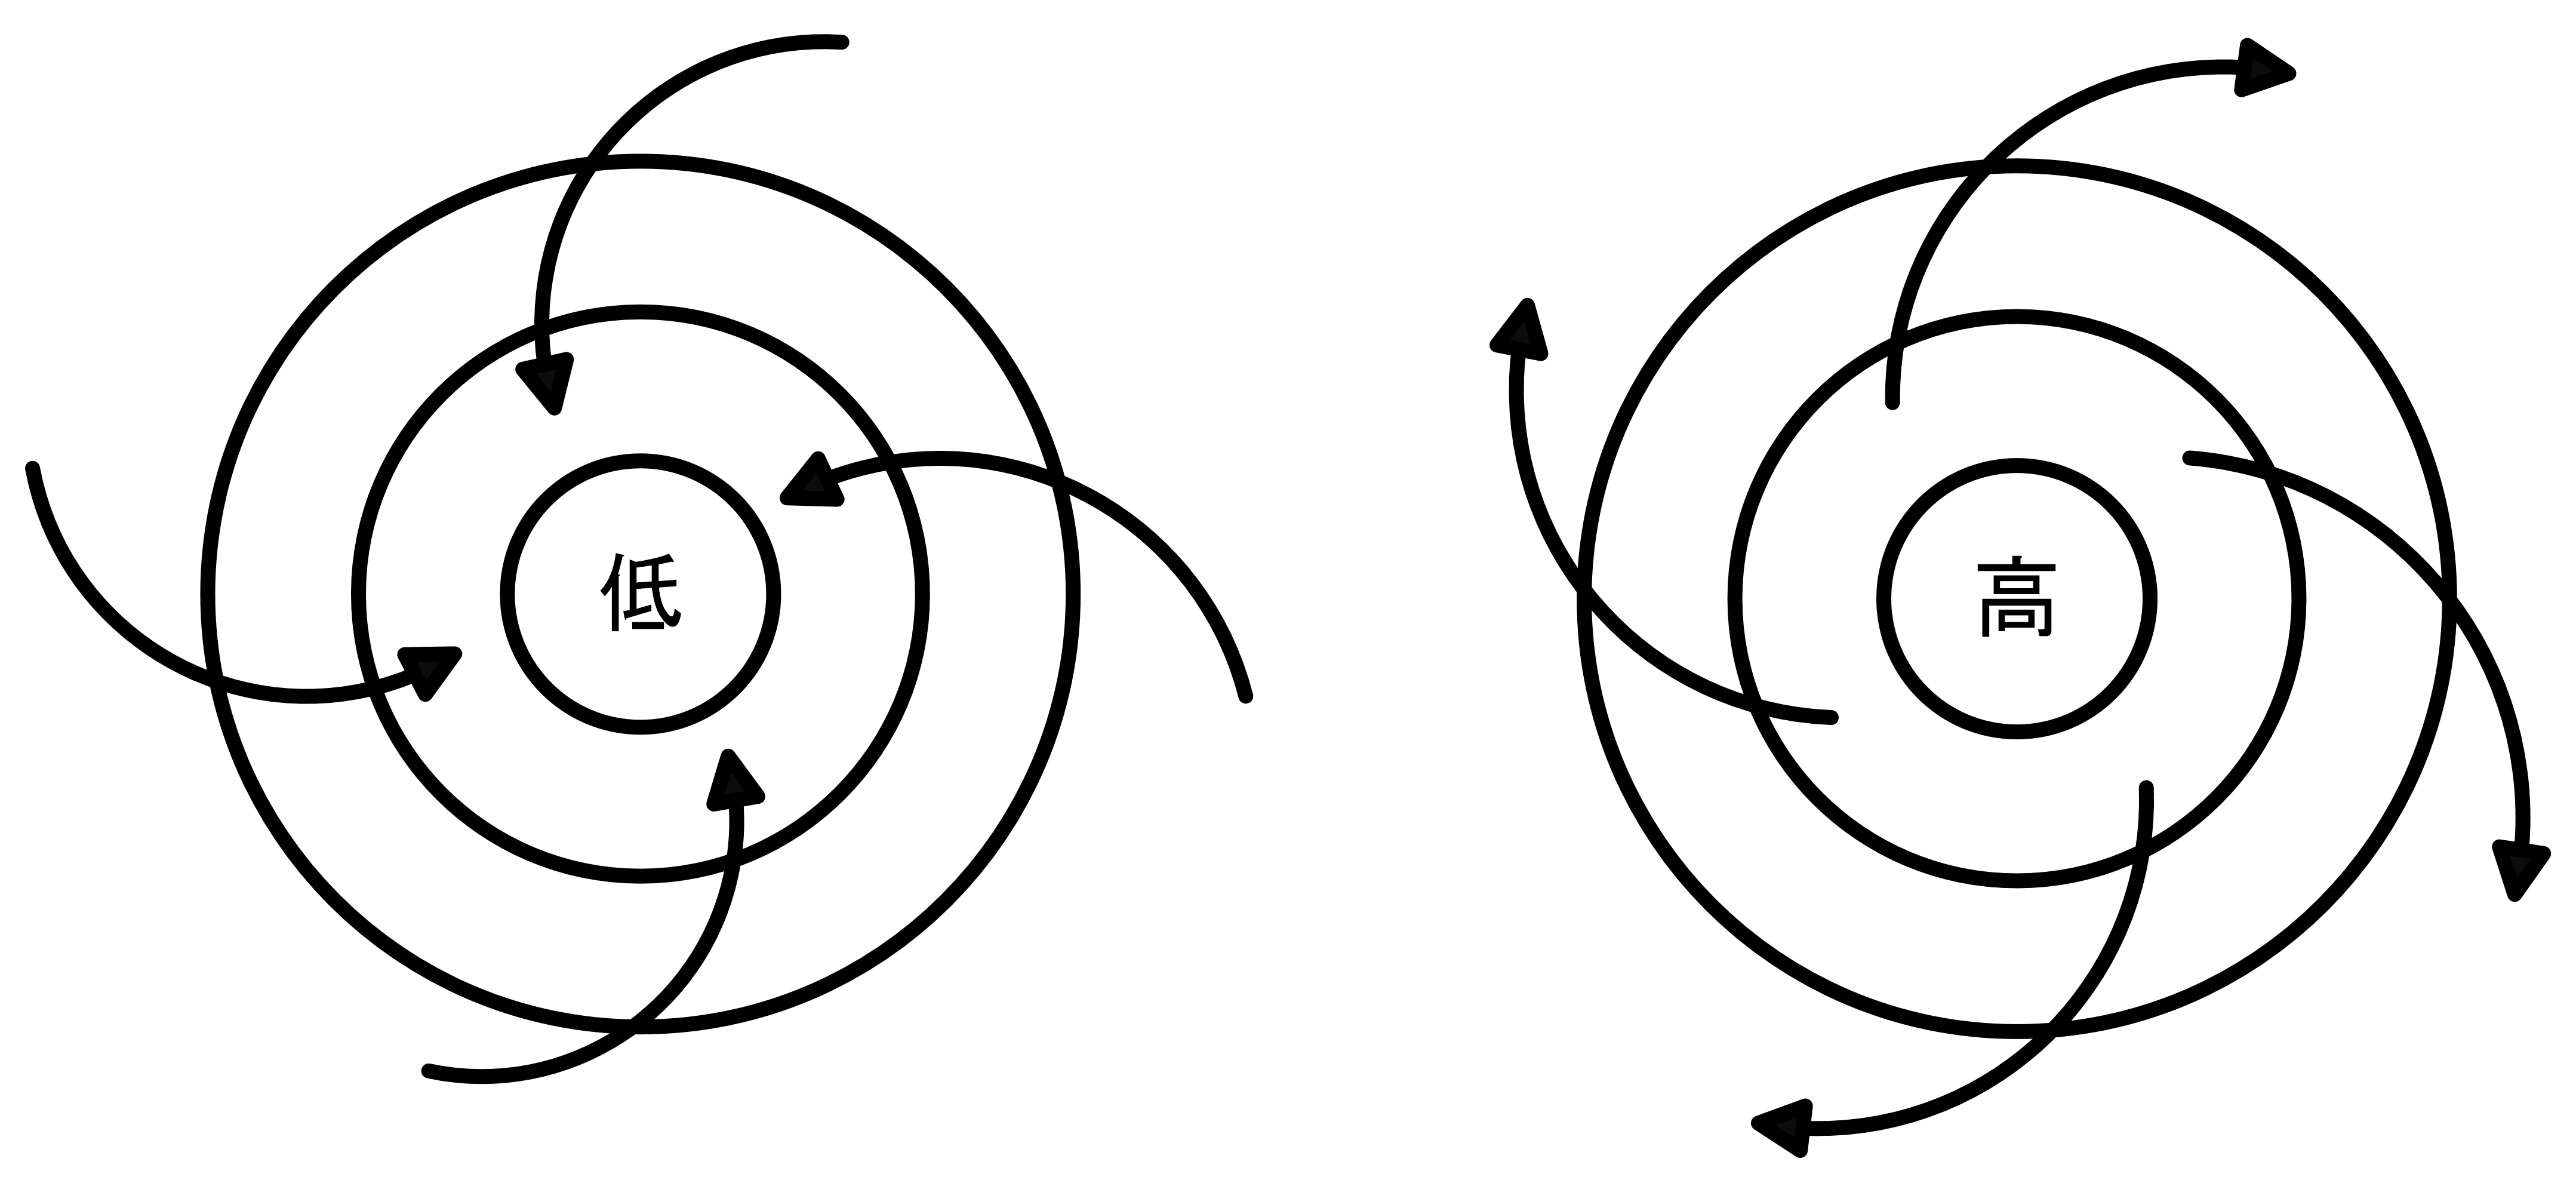
\includegraphics[width=12cm]{img/1-3.png}
        \caption{气旋示意图(北半球)}
    \end{figure}

\end{document}
